\documentclass[tikz,border=5pt]{standalone}
\usepackage{pgfplots}
\usepackage{amsmath}
\pgfplotsset{compat=1.18}

\definecolor{tramU}{HTML}{3F51B5}
\definecolor{tramDos}{HTML}{2E9D5B}
\definecolor{maxim}{HTML}{D32F2F}
\definecolor{minim}{HTML}{D97706}
\definecolor{punt}{HTML}{374151}
\definecolor{asimptota}{HTML}{526CFE}

\begin{document}
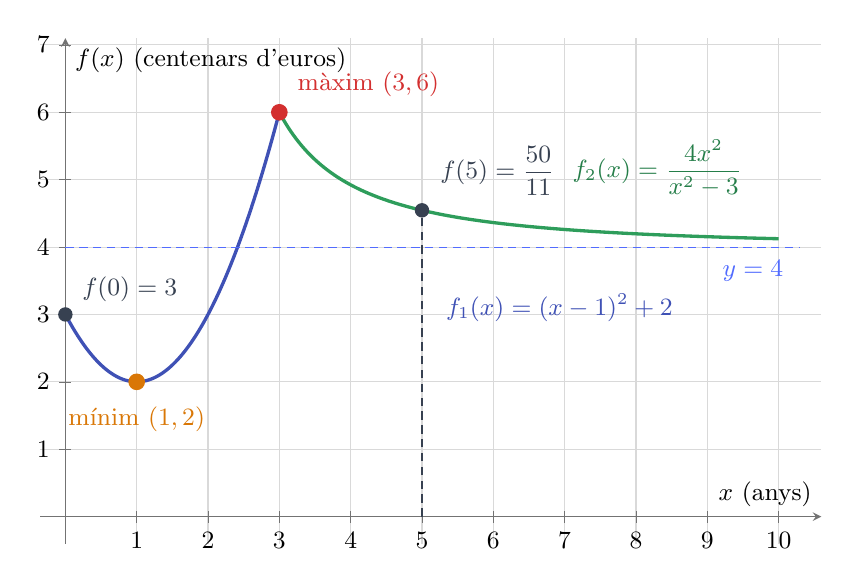
\begin{tikzpicture}
  \begin{axis}[
    width=11.5cm,
    height=8cm,
    axis lines=middle,
    xmin=-0.35,
    xmax=10.6,
    ymin=-0.4,
    ymax=7.1,
    xlabel={$x$ (anys)},
    ylabel={$f(x)$ (centenars d'euros)},
    xtick={0,1,2,3,4,5,6,7,8,9,10},
    ytick={0,1,2,3,4,5,6,7},
    grid=major,
    grid style={black!15},
    axis line style={black!55},
    tick style={black!55},
    tick label style={font=\small},
    label style={font=\small},
    clip=false,
  ]
    \addplot[tramU, very thick, domain=0:3, samples=120]
      {(x-1)^2+2};
    \addplot[tramDos, very thick, domain=3:10, samples=180]
      {4*x^2/(x^2-3)};

    \addplot[asimptota, densely dashed, domain=0:10.3, samples=2]
      {4};

    \draw[punt, densely dashed]
      (axis cs:5,0) -- (axis cs:5,4.54545);

    \addplot[only marks, mark=*, mark size=2.4pt, punt]
      coordinates {(0,3) (5,4.54545)};
    \addplot[only marks, mark=*, mark size=2.8pt, minim]
      coordinates {(1,2)};
    \addplot[only marks, mark=*, mark size=2.8pt, maxim]
      coordinates {(3,6)};

    \node[anchor=south west, text=punt, font=\small]
      at (axis cs:0.1,3.05) {$f(0)=3$};
    \node[anchor=north, text=minim, font=\small]
      at (axis cs:1,1.78) {mínim $(1,2)$};
    \node[anchor=south west, text=maxim, font=\small]
      at (axis cs:3.12,6.08) {màxim $(3,6)$};
    \node[anchor=south west, text=punt, font=\small]
      at (axis cs:5.12,4.62) {$f(5)=\dfrac{50}{11}$};

    \node[anchor=west, text=tramU, font=\small]
      at (axis cs:5.2,3.1) {$f_1(x)=(x-1)^2+2$};
    \node[anchor=south, text=tramDos!80!black, font=\small]
      at (axis cs:8.3,4.6) {$f_2(x)=\dfrac{4x^2}{x^2-3}$};
    \node[anchor=north east, text=asimptota, font=\small]
      at (axis cs:10.2,3.95) {$y=4$};
  \end{axis}
\end{tikzpicture}
\end{document}
